\documentclass[12pt]{article}  
\usepackage{CJK}               %引入CJK宏包
\usepackage{multirow}
\usepackage{indentfirst} %引入首行缩进宏包
\usepackage{fancyhdr} %页眉页脚宏包
\usepackage{graphicx}
\usepackage{subfigure}
\usepackage{float}
\usepackage{graphicx, subfig}
\usepackage{fancyhdr}

\setlength{\parindent}{2em} %设置首行缩进两字节

\begin{document}               %begin与end成对出现
\begin{CJK}{UTF8}{song}        %应用CJK环境
 \pagestyle{fancy}
 \lhead{}
 \chead{}
 \rhead{\bfseries 设计与制造II}
 \lfoot{第二组}
 \cfoot{基于RHex的移动平台设计}
 \rfoot{\thepage}
 \renewcommand{\headrulewidth}{0.4pt}
 \renewcommand{\footrulewidth}{0.4pt}
 
\author{黄威}
\title{电阻应变片电桥特性及应变测试实验}

\renewcommand{\contentsname}{目录} %将content改为目录
\tableofcontents
\newpage

\captionsetup[figure]{labelfont={bf},name={图},labelsep=period}

\section{任务设计书}


\subsection{项目背景}

在一些可能蕴藏着潜在风险的环境中,例如矿洞勘探、洞穴研究、管道维修等,道路情况不清,崎岖的路面令一些先进的勘探仪器机器人也望而却步。突发的情况往往需要人工的操作克服未知的困难、危险的环境,用人命去完成任务成了最为沉重的选择。不可避免的出现了工作人员遇到危险受伤乃至死亡的情况。愿意从事相关行业并具有一定工作经验的从业者较其他行业少得多,他们是社会隐形的财富,倘若失去了他们又是巨大的损失,并且在短时间内难以补充。以上种种,可知恶劣环境中,执行这些任务的机器人是最好的选择。如果能够使这些机器人的行走能力达到人的水平,在诸如爬楼、越过崎岖路面就更有底气执行任务。市面上的机器人因为种种原因没能普及到这类环境中。基于此,我们如果能够设计一款具有强大越障功能的机器人,作为移动平台使用,在其上再附加安装上各种功能模块,就能够实现多重功能,造福于相关行业从业人员。

\subsection{目标人群及特征}
\label{sec:fastguide}
这款移动云台机器人主要针对的是工作在复杂路况环境中的科研人员和相关从业人员,例如抢险救灾的消防员、维修管道的维修工人、地质勘探的科研工作者等等,从事着较为危险的工作,在实际开展工作中面对着难以预料的环境,受限于现有的勘探机器人缺乏强大的越障能力,经常会出现工作失灵的情况,于是工作人员亲自去勘探也就最为常见。总会有未曾预料到的危险情形,每年夺走成百上千的鲜活的生命。
这些相关行业的从业人员的特征是:

\begin{itemize}
\item 工作环境不能保证是平坦的路况,行走其中的崎岖路况常见又难克服。轮式机器人无法在崎岖路面工作,履带式机器人功耗过大,使用时出现硬性碰撞影响其上仪器的工作,稳定性无法得到保证。
\item 没有出色的代替人力的机器人完成相关的工作。咬牙进入危险环境的从业人员极为常见。
\item 精密仪器的价格昂贵,手持往往更令人心安,移动云台的运动缺乏稳定性,可能导致的精密仪器损坏也限制了机器人的广泛应用。移动平台的使用寿命和使用频率很容易大打折扣,甚至被抛弃。
\item 操作复杂,能够进行正常操作往往需要大量的训练和学习,甚至需要专门的人员在旁辅导,完成仪器的操作,无形中增加了使用机器人的成本,降低了机器人的市场竞争力。
\item 现有的移动平台的驱动方式往往只有一种,单一的足式很难保证适应各类环境,亟待整合多种足式运动优势的机器人出现。

\end{itemize}



\subsection{项目目标}
\label{sec:features}
基于此,我们需要设计的一款移动云台机器人应当具有如下的特点:

\subsubsection{平稳性}
\label{sec:requirements}
移动的云台作为勘探仪器的载体,必须要保证移动时的平稳性,避免因为剧烈震动导致精密仪器的损坏,否则从业人员也不放心安装精密仪器在机器人上,考虑到实际需求才能争取这些特征人群的认可

\subsubsection{越障能力}
\label{sec:layout}
强大的越障能力是移动云台机器人胜过其他机器人的保证,也是项目在进行设计和组装过程中尽力去完成的一方面。为此设计组先后考虑了多自由度足式、履带式等多种驱动方式,最终敲定了“C”型足。这款足式侧面酷似大写的”C”,具有出色的越障功能。

\subsubsection{传动稳定}
\label{sec:format}

很多的机器人依靠控制系统来实现稳定的传动和精准的控制,这固然是机器人的一大发展趋势,可是忽视了复杂环境中对于机器人的严苛考验、单单依靠控制系统完成平稳传动又是不太现实的,利用齿轮、同步带等机械结构实现稳定可靠的传动,对提高机器人的生存能力和工作寿命都是十分有意义的。
\subsubsection{负载能力}
\label{sec:format}

作为直接连接功能模块的机器人,不仅要保证能够独自行走,还要保证接入功能模块,也同样能够行走。这就给机器人的材料选择提出了更高的要求,零件的强度足够安装上功能模块,不锈钢、铝合金是现有的选择,未来还可以使用高性能复合材料,降低机器人的自重的同时,提高了机器人的负载能力。
\subsubsection{操作简便}
\label{sec:format}

例如管道维修工等使用机器人也是为了简便,如果操作复杂,甚至是只能专业人员去操控,无疑增加了工作成本,也会使设计产品失去产品竞争力。做到移动云台机器人的简便操作,不仅会降低工作成本,也会降低后续维修工作的难度,开拓更为广阔的市场前景。
\subsubsection{平地行驶}
\label{sec:format}

不仅要能够实现越障功能,移动平台机器人在较为平坦的路面上,具有出色的行走能力同样重要。速度太慢而被抛弃的机器人并不在少数。

\subsection{市场现有产品的优劣分析}
\subsubsection{轮式移动平台机器人}
\renewcommand {\thefigure} {\thesubsection{}.\arabic{figure}}
\begin{figure}[H]
\centering
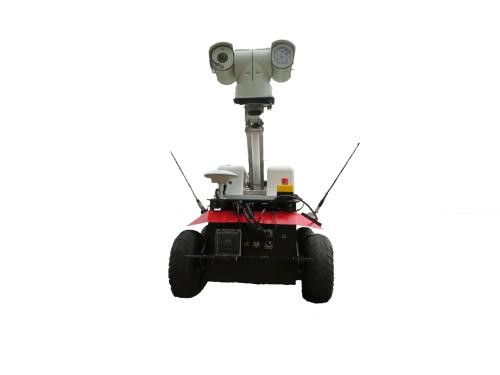
\includegraphics[width=.8\textwidth]{chap1//fig1.jpg}
\caption{移动监控机器人}
\end{figure}
\begin{figure}[H]
\centering
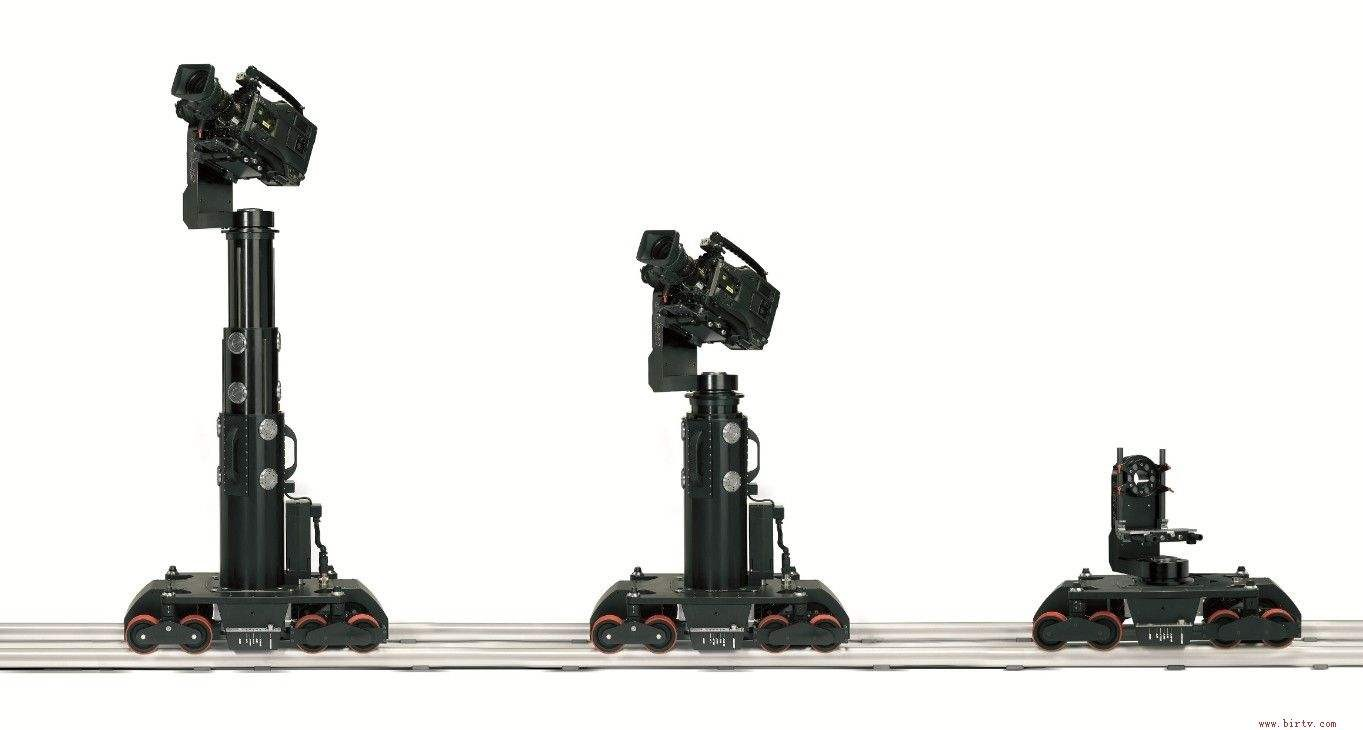
\includegraphics[width=.8\textwidth]{chap1//fig2.jpg}
\caption{连接测量模块的轮式机器人}
\end{figure}
优点:移动平稳而快速,适用于较为平坦的路面进行执行各类任务。\par
缺点:不能翻越较为崎岖的路面,适应性较差,应用范围受到限制。

\subsubsection{履带式移动平台机器人}
\begin{figure}[H]
\centering
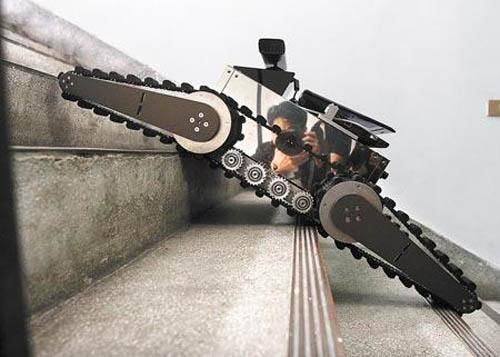
\includegraphics[width=.8\textwidth]{chap1//fig3.jpg}
\caption{“NTNU CIR-I”的履带式机器人}
\end{figure}
优点:相较于轮式在越障能力方面有了较为明显的优势。操作简便,运行时也足够平稳,负载能力较高。\par
缺点:运行速度慢,不适合平坦地形的勘探,降低了勘探效率。重量大,需要的功率大,一般电机难以驱动。缓冲少,因而零件的磨损速度快。

\subsubsection{“C”型足式机器人}
\begin{figure}[H]
\centering
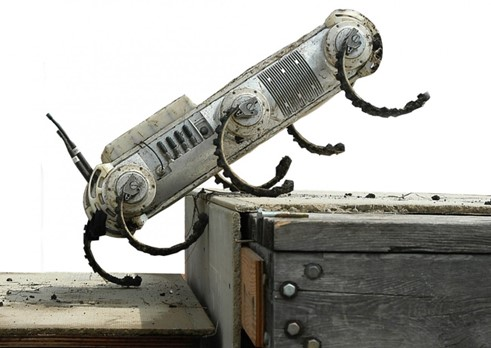
\includegraphics[width=.8\textwidth]{chap1//fig4.jpg}
\caption{“Rhex”机器人}
\end{figure}
优点:车身应用了复合材料,重量较轻,C字型足给予了移动平台强大的越障能力,同时保证了足够的缓冲,运行较为平稳。\par
缺点:车身材料、驱动电机等价格昂贵,不具有价格优势。内部控制系统较为复杂,维修成本较高。平坦地面运动不具优势。

\par
基于此,项目组在原有的C字型足式机器人的基础上,用齿轮系前轮替换了前轮C字型足。创造性的实现了两种运动形式,在平坦地面使用轮式发挥轮式的优势,速度足够快。在崎岖路面使用C字型足作为驱动轮,保证了越障能力,同时运动足够平稳。


\section{机械结构设计}
\subsection{功能分解}
\subsubsection{C型足传动}
C形足传动的设计使六足机器人能能够实现足式前进。\par
采用单输入多输出的形式,能够利用一个电机控制单边的三个C形足。同时,利用机械结构而不是电控来实现C形足的一种急回效应,缩短C形足在空中的无功时间。
\subsubsection{齿轮系驱动前轮}
	齿轮系驱动前轮的设计使六足机器人能实现轮式、足式两种运动模式的自由切换。\par
	足式运动模式下,通过同步带轮传动,可以实现与普通C型足一样的足式效果。同时,由于采用平行四杆与齿轮系相结合的结构,加上柔性约束后,实现了主动轮到从动轮的轴距可变,且能承受一定的冲击载荷,可适应复杂路面状况。\par
	轮式运动模式下,同步轮锁死,单独控制前轮驱动电机驱动齿轮组,可将电机转矩由机体内部传递到驱动前轮足底的轮子上,使其能以轮式在平滑路面行进。
	
\subsection{整体结构展示}
如下图,分别为整体结构的实物图和建模图。
\renewcommand {\thefigure} {\thesubsection{}.\arabic{figure}}
\begin{figure}[H]
\centering
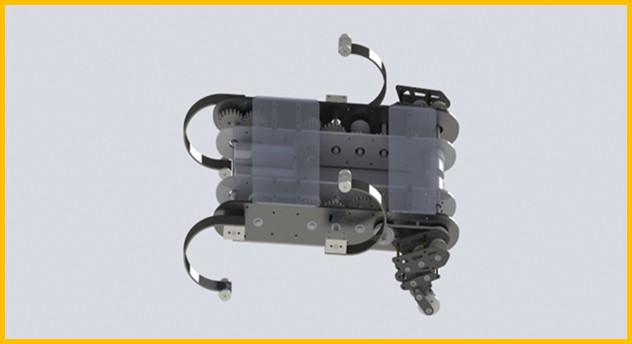
\includegraphics[width=.8\textwidth]{chap2//fig2.jpg}
\caption{主体部分-模型渲染图}
\end{figure}
\begin{figure}[H]
\centering
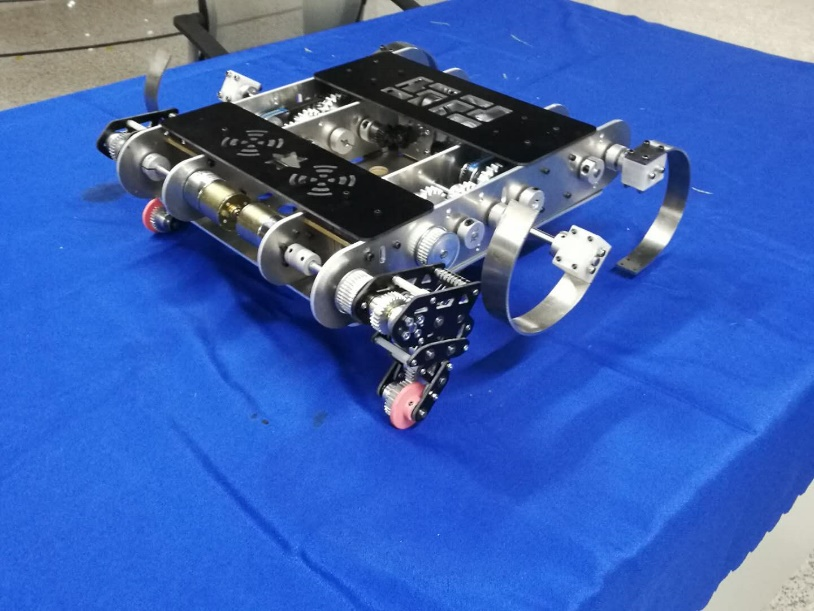
\includegraphics[width=.8\textwidth]{chap2//fig1.jpg}
\caption{主体部分-实物搭建图}
\end{figure}
\begin{figure}[H]
\centering
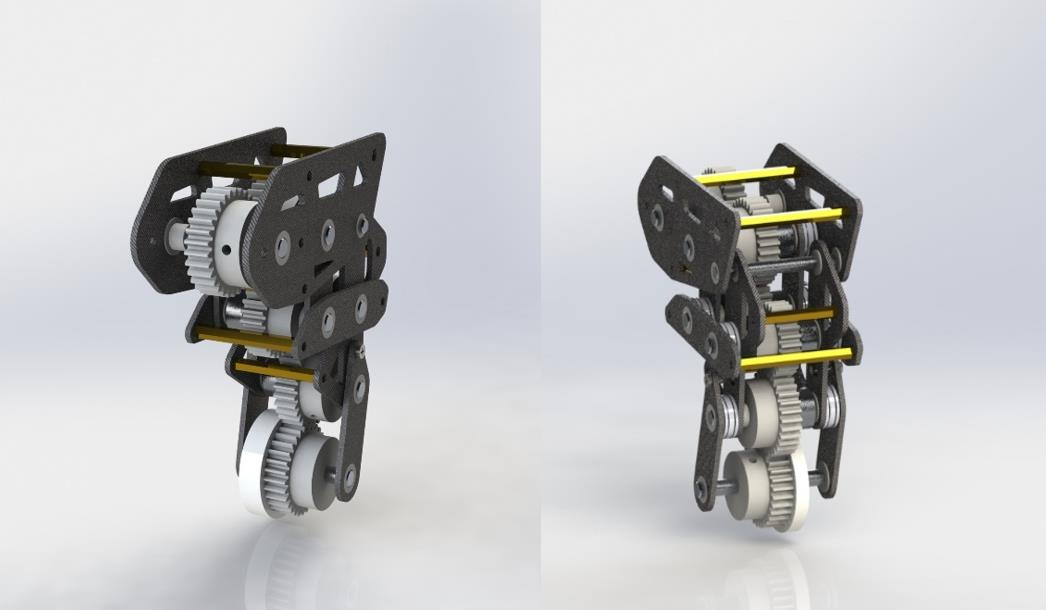
\includegraphics[width=.8\textwidth]{chap2//figa.jpg}
\caption{齿轮系驱动前足-模型渲染图}
\end{figure}
\begin{figure}[H]
\centering
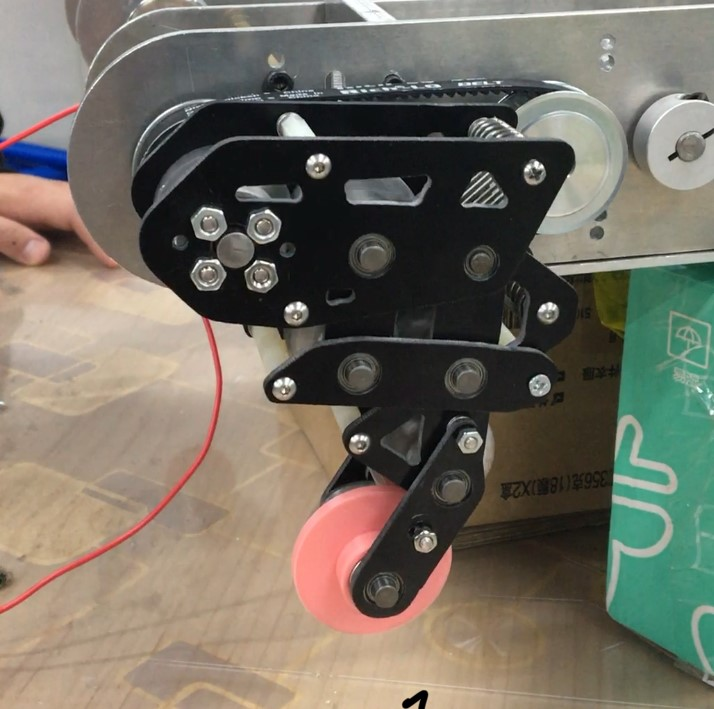
\includegraphics[width=.6\textwidth]{chap2//figb.jpg}
\caption{齿轮系驱动前足-实物搭建图}
\end{figure}

\subsection{结构设计}
\subsubsection{C形足传动设计}
主体传动结构主要用以实现移动平台的足式运动。需要实现的功能有一下两点:\par
\begin{itemize}
\item 实现单电机三输出的驱动效果。
\item 实现C形足的急回效应(在空中的无功过程用时短,与地面接触的有功过程停留时间更久)。
\end{itemize}

\textbf{2.3.1.1 C形足传动框架的搭建}\par
 如图a,为单边C形足的主体框架爆炸图,由三块骨架板和两块轴固定板构成,两块轴固定板与骨架板通过侧边的两个螺纹孔进行连接固定。\par
如图b,为主体框架的整合图,在骨架板的上下底面分别有两个螺纹孔,使得主体传动机构可以和删改底板进行固定。
\begin{figure}[H]
%\centering
\subfigure[框架爆炸图]{
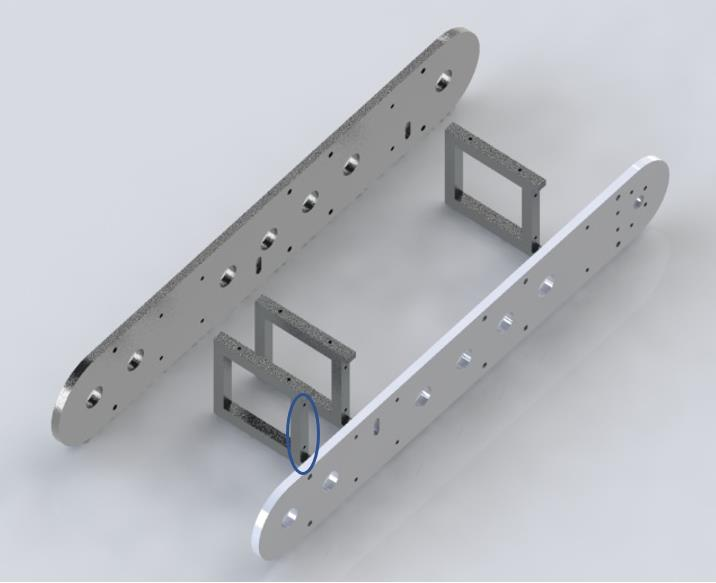
\includegraphics[width=.45\textwidth]{chap2//fig3.jpg}
%\caption{fig1}
}
\quad
\subfigure[框架整合图]{
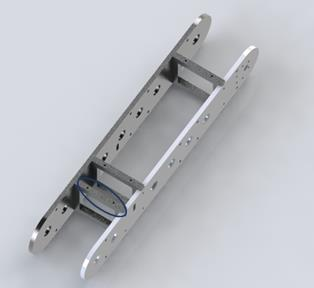
\includegraphics[width=.4\textwidth]{chap2//fig4.jpg}
%\caption{fig1}
}
\quad
\caption{C形足传动框架}
\end{figure}
\textbf{2.3.1.2 锥齿轮的设计}\par
 使用锥齿轮实现交错轴的传动,节省横向空间,减小整体设计的横向尺寸。
 \begin{figure}[H]
%\centering
\subfigure[锥齿轮传动结构图]{
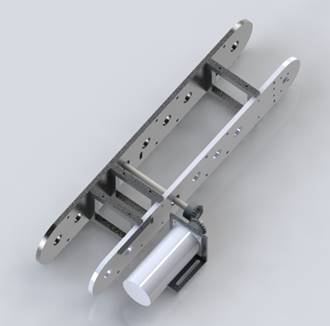
\includegraphics[width=.45\textwidth]{chap2//fig5.jpg}
%\caption{fig1}
}
\quad
\subfigure[横向尺寸示意图]{
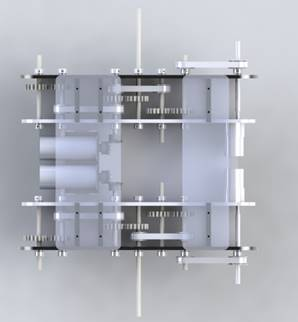
\includegraphics[width=.4\textwidth]{chap2//fig6.jpg}
%\caption{fig1}
}
\quad
\caption{锥齿轮设计}
\end{figure}
\textbf{2.3.1.3 同步轮的设计}\par
 使用同步轮将一根轴的输出量传递到三根轴,实现一输入,三输出的效果
 \begin{figure}[H]
%\centering
\subfigure[同步轮传动结构图]{
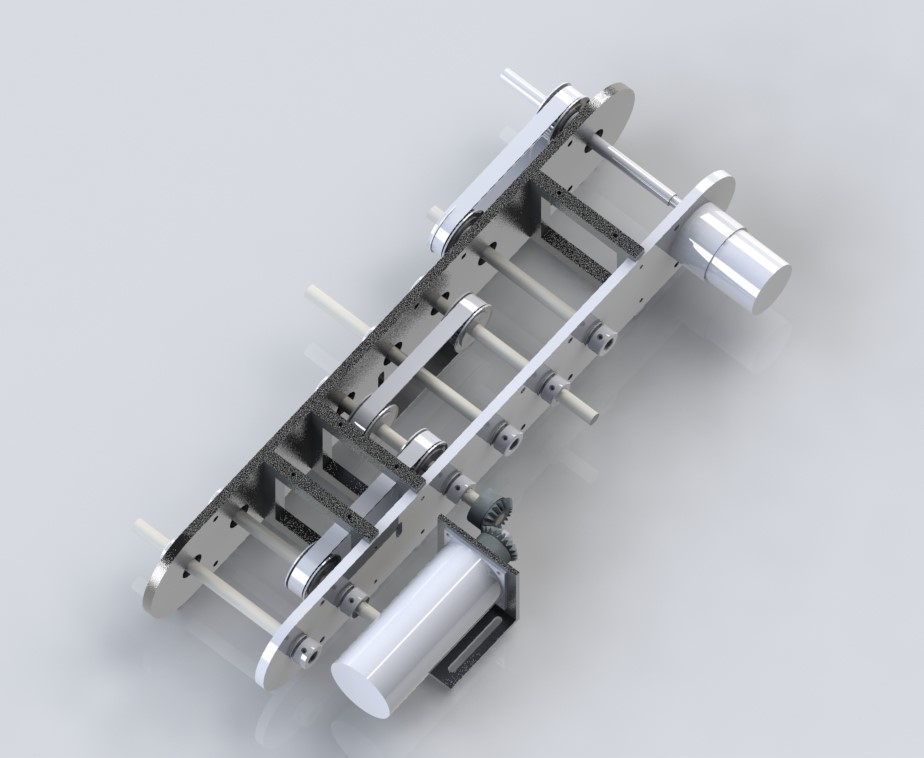
\includegraphics[width=.5\textwidth]{chap2//fig7.jpg}
%\caption{fig1}
}
\quad
\subfigure[三输出示意图]{
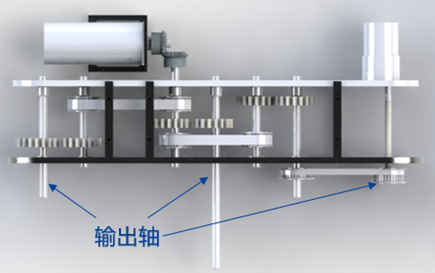
\includegraphics[width=.5\textwidth]{chap2//fig8.png}
%\caption{fig1}
}
\quad
\caption{同步轮设计}
\end{figure}
\textbf{2.3.1.4 椭圆齿轮的设计}\par
 使用椭圆齿轮,实现变传动比的传动,即一种缩短空中无功时间的急回特性。
 \begin{figure}[H]
%\centering
\subfigure[椭圆齿轮传动结构图]{
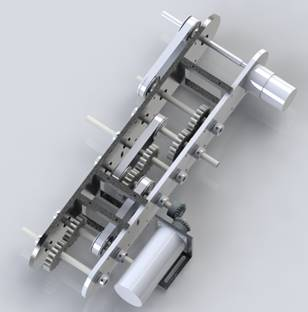
\includegraphics[width=.5\textwidth]{chap2//fig9.jpg}
%\caption{fig1}
}
\quad
\subfigure[椭圆齿轮]{
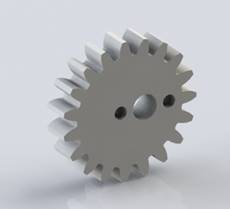
\includegraphics[width=.5\textwidth]{chap2//fig10.jpg}
%\caption{fig1}
}
\quad
\caption{椭圆齿轮设计}
\end{figure}
\subsubsection{齿轮系驱动前轮}
\textbf{2.3.2.1 1,	齿轮系设计}\par
 齿轮系驱动前轮主体设计结合了采用齿轮系与平行四杆,从而实现主动轮到从动轮之间的轴距可根据不同状态调节。
 \begin{figure}[H]
\centering
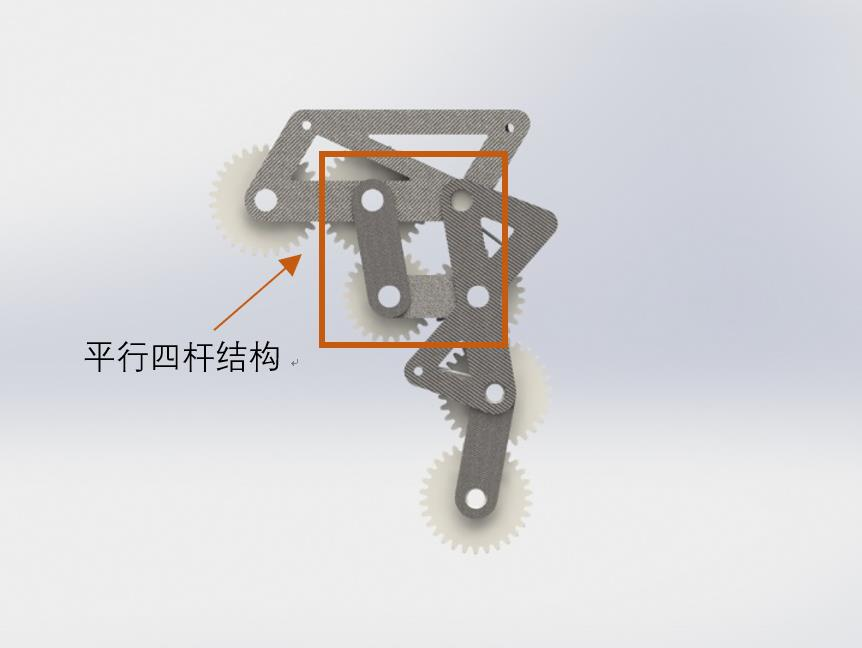
\includegraphics[width=.6\textwidth]{chap2//figc.jpg}
\caption{结构侧视图}
\end{figure}
足式模式下,齿轮系驱动前足需作为普通C型足使用,其设计尺寸应与普通C型足一致,因此最终选用大小齿轮分别为1模25齿和30齿,在骨架约束下可以满足半圆直径120mm的要求。同时,主体骨架利用六角铜柱进行固定,保证齿轮系驱动前轮有足够的强度,可承受一定冲击。
 \begin{figure}[H]
%\centering
\subfigure[齿轮系内部结构]{
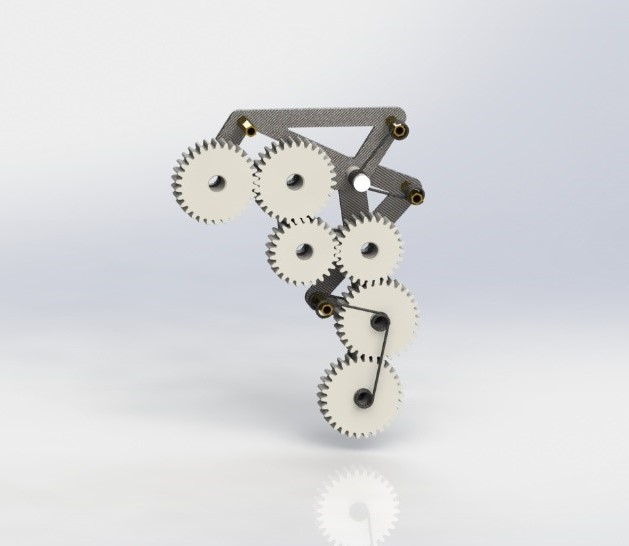
\includegraphics[width=.5\textwidth]{chap2//figd.jpg}
%\caption{fig1}
}
\quad
\subfigure[六角铜柱安装]{
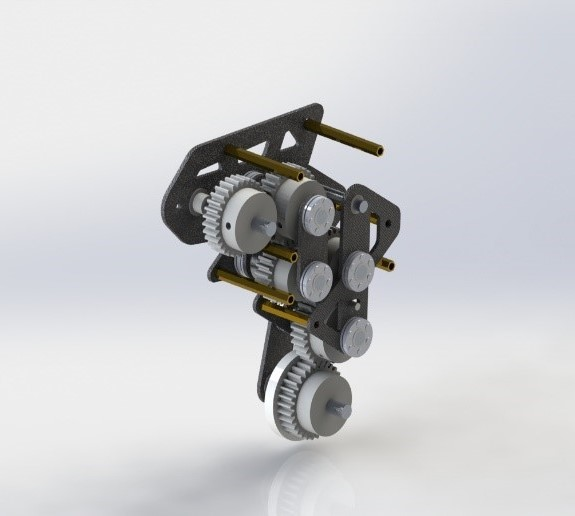
\includegraphics[width=.5\textwidth]{chap2//fige.jpg}
%\caption{fig1}
}
\quad
\caption{齿轮系驱动前足剖面图}
\end{figure}
\textbf{2.3.2.2	柔性约束}\par
由于作为普通C型足刨地行进时,前轮会受到较大的冲击载荷,需要添加适当的柔性约束保证内部齿轮系不受到破坏。因此主体骨架中采用了平行四杆结构,系统增加一个自由度,同时添加扭簧作为约束,实现避震功能。因为单独定做合适角度尺寸的扭簧价格高昂,所以提前选定好了一款满足前轮扭力需求的标准件扭簧后,根据其型号修改了骨架结构。最终,实现了正常状况下齿轮系的相对固定形态,而受到冲击时也可实现一定的弹性变形。同时,轮式运动模式下该柔性约束也可以作为悬挂架进行减震。
 \begin{figure}[H]
%\centering
\subfigure[模型图]{
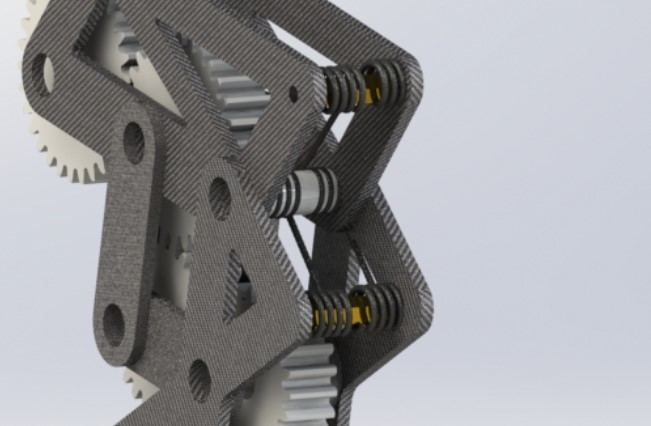
\includegraphics[width=.5\textwidth]{chap2//figf.jpg}
%\caption{fig1}
}
\quad
\subfigure[实物图]{
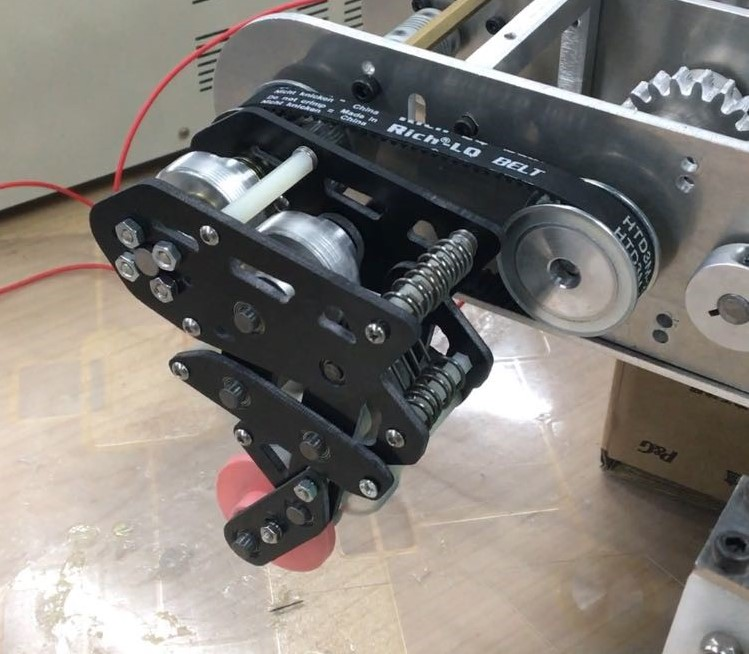
\includegraphics[width=.5\textwidth]{chap2//figg.jpg}
%\caption{fig1}
}
\quad
\caption{扭簧安装示意}
\end{figure}

\textbf{2.3.2.3	装配设计}\par
因齿轮系驱动前足所使用的零部件较多,且尺寸较小,所以在设计过程中考虑了安装的可行性,并对装配过程进行了优化、模拟。最终装配时,先完成两块基本齿轮组件的安装,再将两个模块固定在骨架即可,大大简化了装配过程。
\begin{figure}[H]
%\centering
\subfigure[组块1]{
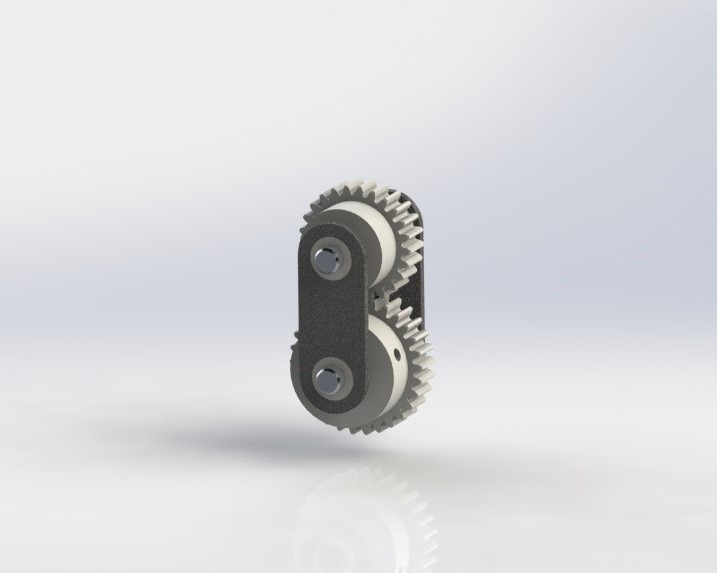
\includegraphics[width=.5\textwidth]{chap2//figh.jpg}
%\caption{fig1}
}
\quad
\subfigure[组块2]{
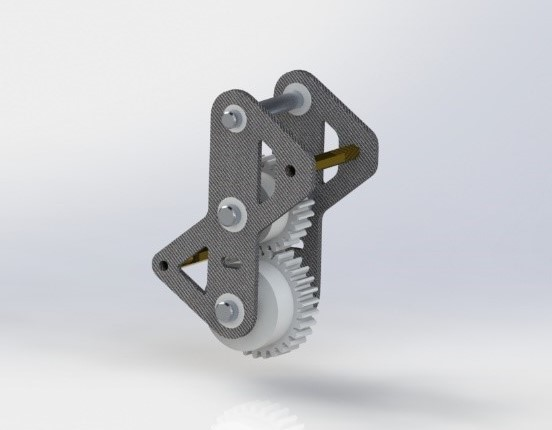
\includegraphics[width=.5\textwidth]{chap2//figi.jpg}
\quad
}
\caption{装配示意-组块分解}
\end{figure}

 \begin{figure}[H]
\centering
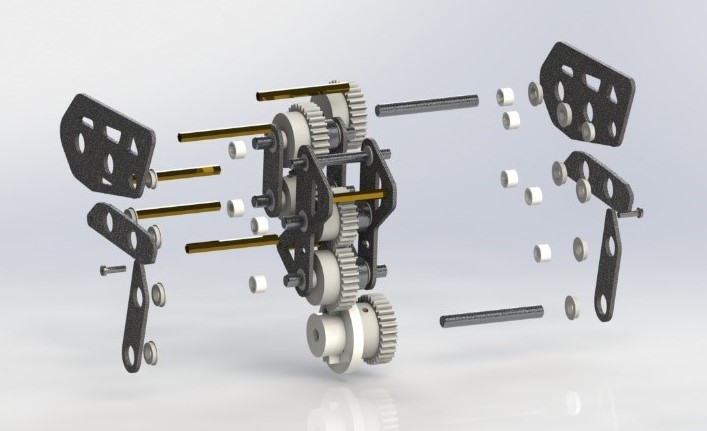
\includegraphics[width=.9\textwidth]{chap2//figj.jpg}
\caption{装配示意-总装爆炸图}
\end{figure}

此外,底轮和扭簧安装块都设计了滑槽孔位,方便利用改变螺丝位置调整前轮C型足的尺寸和形态。
 \begin{figure}[H]
\centering
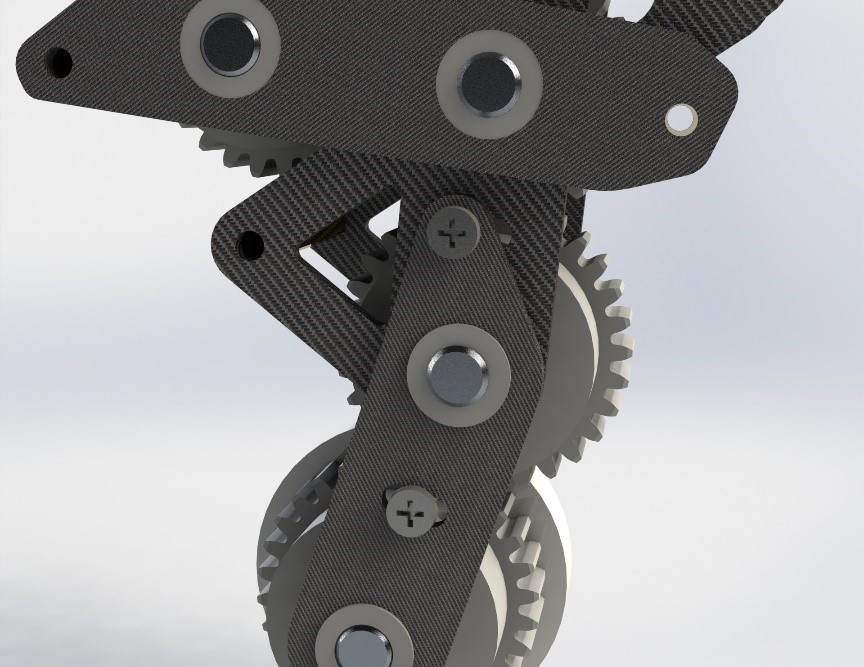
\includegraphics[width=.6\textwidth]{chap2//figk.jpg}
\caption{调节孔位}
\end{figure}
\subsubsection{整体装配}
\textbf{2.3.3.1	前轮的轮式、足式切换}\par
\begin{itemize}
\item 利用同步轮实现齿轮系前轮的足式运动。
\item 利用电机驱动齿轮系带动C形足末端的小轮实现轮式运动。
\end{itemize}
从动同步轮与齿轮系前足中间用螺丝连接,实现运动的传递;同时从动同步轮采用惰轮,即中间套有轴承,防止足式驱动轴与同步轮运动的牵连。
 \begin{figure}[H]
\centering
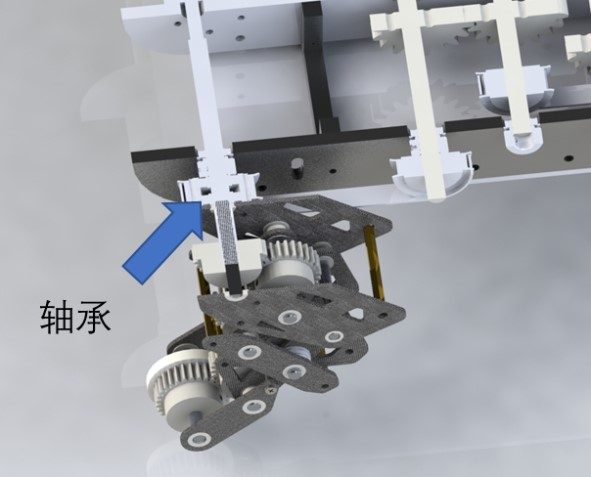
\includegraphics[width=.6\textwidth]{chap2//fig21.jpg}
\caption{轴承示意}
\end{figure}
 \begin{figure}[H]
\centering
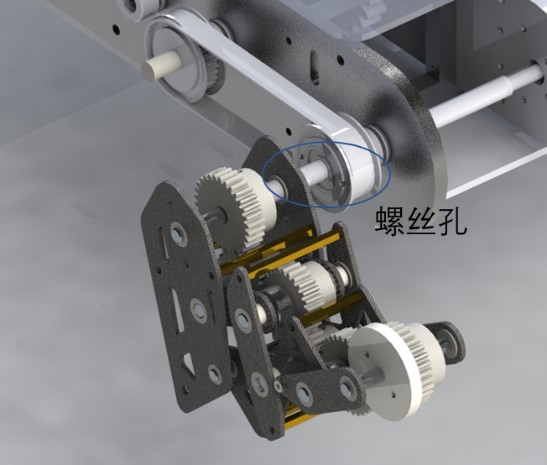
\includegraphics[width=.6\textwidth]{chap2//fig22.jpg}
\caption{螺丝孔示意}
\end{figure}

\textbf{2.3.3.2	C形足安装要求}\par
由于三边三个C形足的足式运动依靠单个电机驱动,所以三个C形足之间的相位差是一定的,为了保证运行过程中平台的相对平稳,选择在安装时将中部C形足相对前后C形足差180°安装,保证足式运动时至少三个C形足着地。
    在轮式前行的过程中,则依靠前后四轮着地保证平台稳定。
 \begin{figure}[H]
\centering
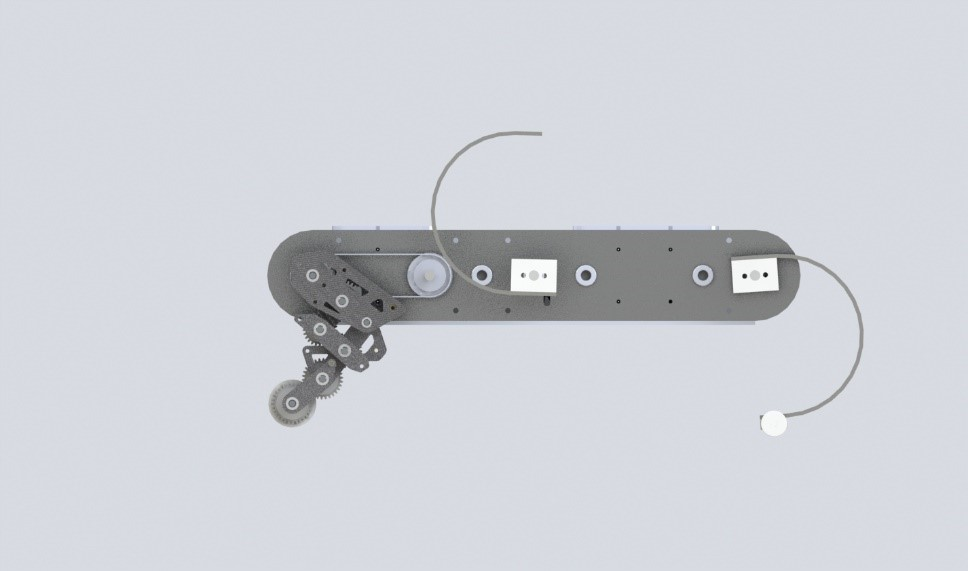
\includegraphics[width=.65\textwidth]{chap2//fig23.jpg}
\caption{C形足安装要求}
\end{figure}

\textbf{2.3.3.3	电路元件安置}\par
考虑整体的封装性和外观,根据电池、电机驱动模块控制板、及电路的大概尺寸,设计时预留了电路元件的安置位置。
 \begin{figure}[H]
\centering
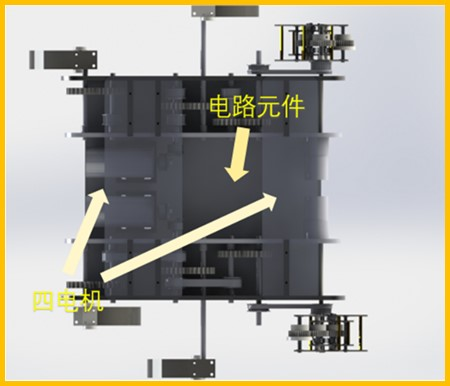
\includegraphics[width=.55\textwidth]{chap2//fig24.jpg}
\caption{空间布置}
\end{figure}


\section{主要结构的选型和绘制}

\subsection{椭圆齿轮的绘制}
非圆齿轮机构可实现非匀速比传动,且具有结构紧凑、传动平稳和易实现动平衡等优点。但因每个齿廓不尽相同,设计比较复杂。\par
首先,设计节曲线(相似于齿轮中节圆的概念),长半轴a=20mm(由轴距确定),短半轴b=19.36mm,偏距e=0.25,再确定椭圆齿轮的齿数(便于啮合通常为奇数齿),Z=19,此时可得到齿轮模数m=C*pi/Z(非标准模数)。\par
其次,将基椭圆19等分,采用“折算齿数”的方法,即A等分点处的曲率半径为ρA,则A处齿形的折算齿数ZA=2ρA/m。按设计手册分别按齿顶高: ha=m,齿根高:hf=1.25m在节椭圆内外作齿顶椭圆和齿根椭圆。通过作图软件CAXA绘制得到齿形草图(如图a所示)。\par
最后通过SolidWorks建模出图(如图b所示)。
\begin{figure}[H]
%\centering
\subfigure[CAXA绘制齿廓]{
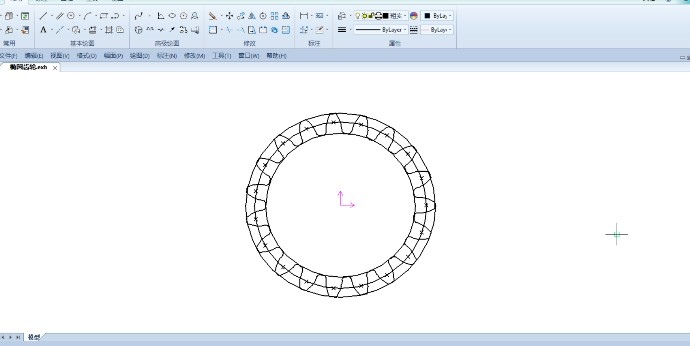
\includegraphics[width=.5\textwidth]{chap3//fig1.jpg}
%\caption{fig1}
}
\quad
\subfigure[SolidWorks绘制齿轮]{
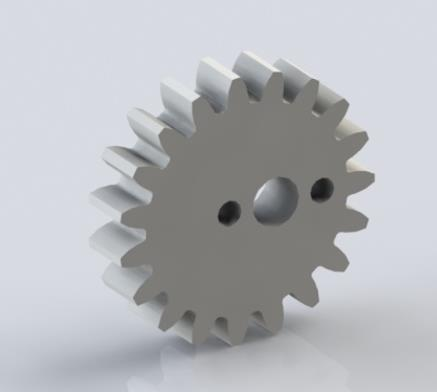
\includegraphics[width=.45\textwidth]{chap3//fig2.jpg}
\quad
}
\caption{椭圆齿轮}
\end{figure}

\subsection{C形足的选材}
通过静应力分析,发现在承受30N静载荷的情况下,铝合金已经出现了屈服,所以最终选用304不锈钢作为C形足的材料。
\begin{figure}[H]
%\centering
\subfigure[304不锈钢]{
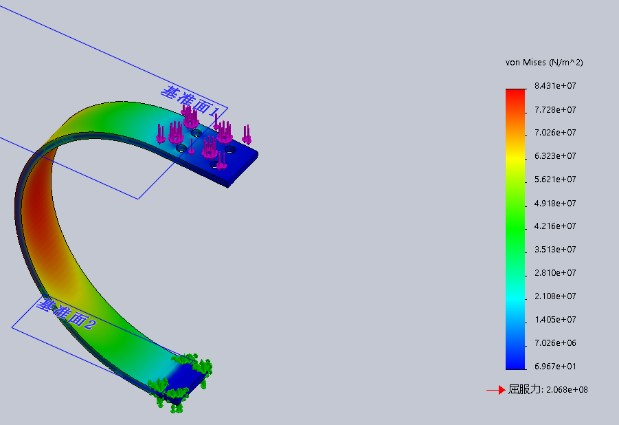
\includegraphics[width=.5\textwidth]{chap3//fig3.jpg}
%\caption{fig1}
}
\quad
\subfigure[6061铝合金]{
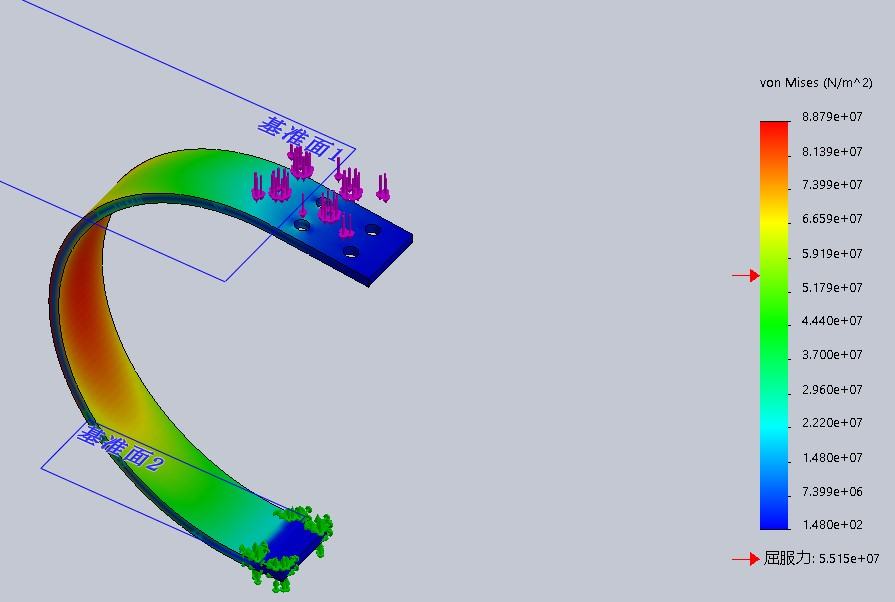
\includegraphics[width=.5\textwidth]{chap3//fig4.jpg}
\quad
}
\caption{静应力分析}
\end{figure}

\subsection{齿轮选型}
为了保证齿轮系驱动前足设计尺寸与其他普通C型足一致,初定齿轮大小齿轮型号分别为1模25齿和30齿,由于设计的齿轮系驱动前轮为开式传动,因此需要进行弯曲强度校核。\par
所选用齿轮为1模25齿和30齿的凸台圆柱直齿轮,材质选用铝合金。其基本参数以及所受力矩如下。\par
\begin{table}[!htbp]
\centering
%\caption{R1R7组成半桥}
\begin{tabular}{|c|c|c|c|} % 通过添加 | 来表示是否需要绘制竖线
\hline %绘制横线
额定力矩T1/kg*cm&模数m&齿数z1&齿宽b/mm\\
\hline
2.25&1&25/30&8\\
\hline
\end{tabular}
\end{table}
同时,根据使用状况以及结构选定校核修正系数。其中,原动机为直流电机且轮式使用下载荷较为均匀,故载荷系数k取1.2;齿型系数YF由齿数查图可得YF=2.7;应力集中系数YS
由图可得YS=1.6。由公式\par
$$\sigma _ { \mathrm { F } } = \frac { 2 K T _ { 1 } Y _ { \mathrm { Fa } } Y _ { \mathrm { Sa } } } { b d _ { 1 } m } = \frac { 2 K T _ { 1 } Y _ { \mathrm { Fa } } Y _ { \mathrm { Sa } } } { b m ^ { 2 } z _ { 1 } } $$
可计算得弯曲应力$\sigma _ { \mathrm { F } } $为21.87MPa,而铝合金弯曲疲劳强度约为200MPa,取安全系数S=2,得许用弯曲应力为$\left[ \sigma _ { \mathrm { F } } \right]$100MPa。因此可以满足使用需求。

\subsection{主电机选型}
选择工况为翻越10cm高台阶进行扭矩的校核计算。\par
首先,为了保证平台的平稳前进,电机的转速需要达到200rpm。\par
其次,整车重量为8kg,假定整车重心位于主体的几何中心。假定地面的摩擦系数为0.5,为了实现小车能够顺利爬上台阶(如图3.4.1),FN1$\approx$4 kg,FN2$\approx$4kg,f1=f2=2kg,则两处需要产生的扭矩之和约为2.5N.m+1.5 N.m$\approx$4N.m,这些扭矩由两个主动电机共同承担,则单个电机的连续输出扭矩至少需要达到2N.m。\par
而原本选择的直流有刷电机的最大输出扭矩只有1.4N.m,远没有达到需求值,使得最终无法实现稳定的足式前进。\par
打算采用DJI-M3508直流无刷电机,其具体参数如图所示,各参数均可满足需求,并留有很大的安全裕量。
 \begin{figure}[H]
\centering
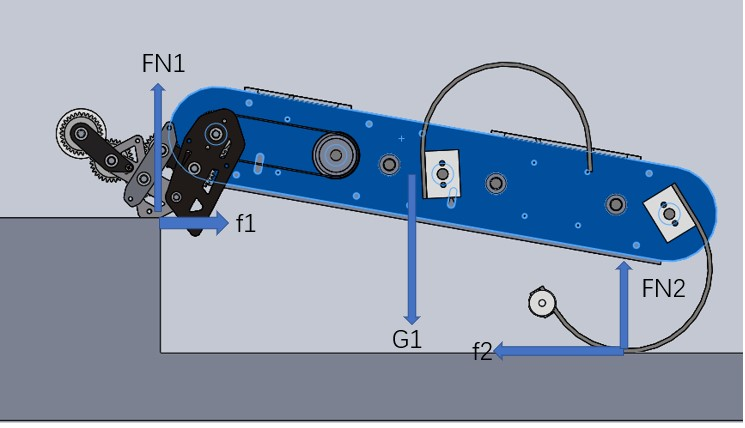
\includegraphics[width=.8\textwidth]{chap3//fig6.jpg}
\caption{爬台阶受力图}
\end{figure}
 \begin{figure}[H]
\centering
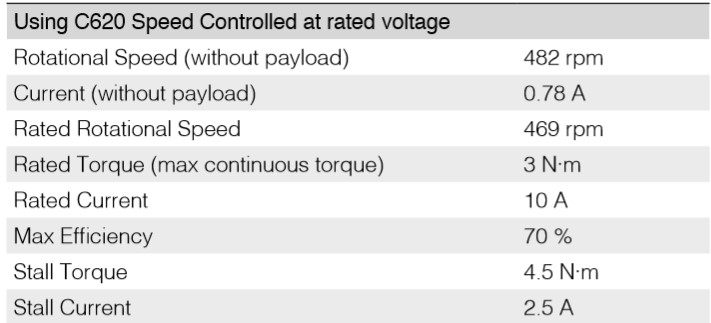
\includegraphics[width=.8\textwidth]{chap3//fig7.jpg}
\caption{电机参数}
\end{figure}

\subsection{同步轮选型}
根据电机的P-T曲线,可以得知,在扭矩为1.5N.m时,其功率约为30W。
 \begin{figure}[H]
\centering
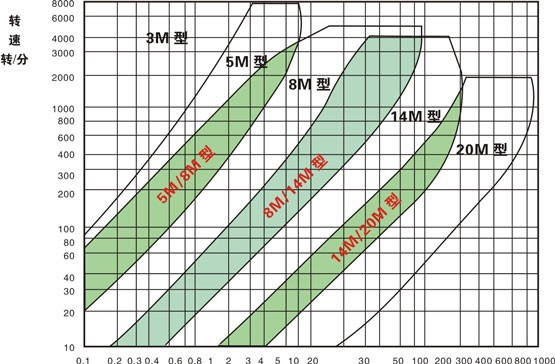
\includegraphics[width=.8\textwidth]{chap3//fig9.jpg}
\caption{电机P-T曲线}
\end{figure}
根据同步轮选型图,可以发现200rpm,0.03kW时,选择3M型同步轮就可以满足要求。


\section{加工件、其余零部件}
\subsection{加工件尺寸标注}
 \begin{figure}[H]
\centering
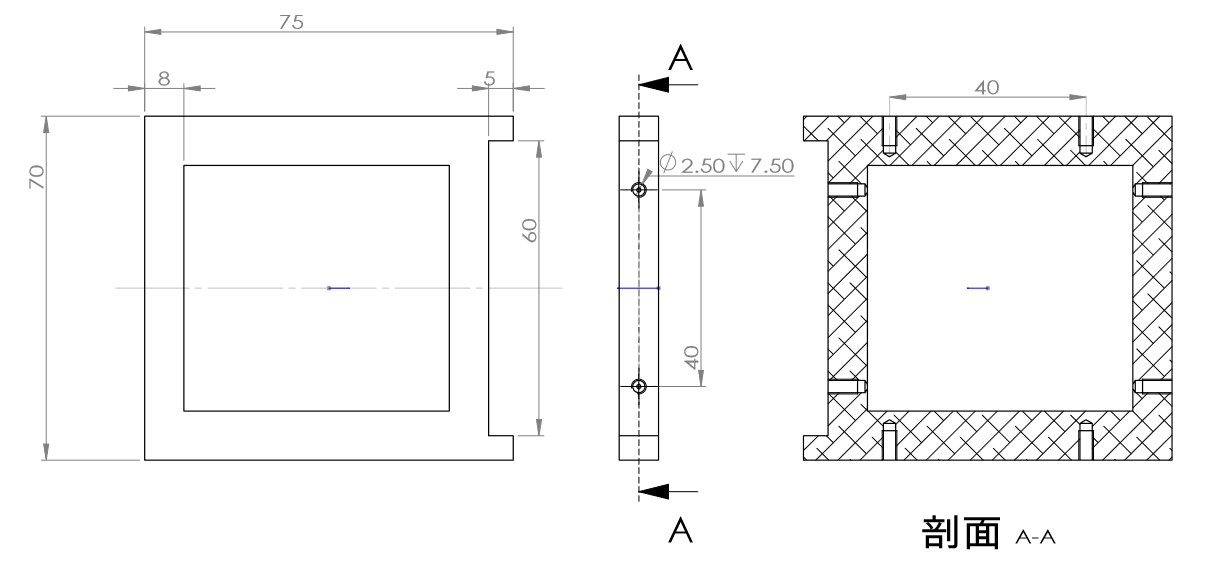
\includegraphics[width=.9\textwidth]{chap4//Fig1.jpg}
\caption{骨架板}
\end{figure}
 \begin{figure}[H]
\centering
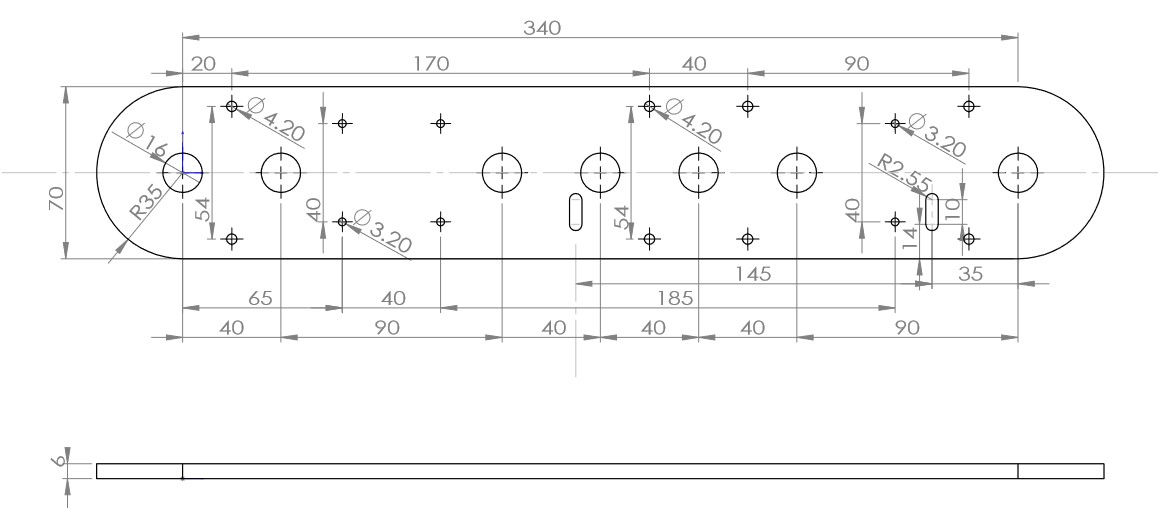
\includegraphics[width=.9\textwidth]{chap4//Fig2.jpg}
\caption{轴固定外板}
\end{figure}
 \begin{figure}[H]
\centering
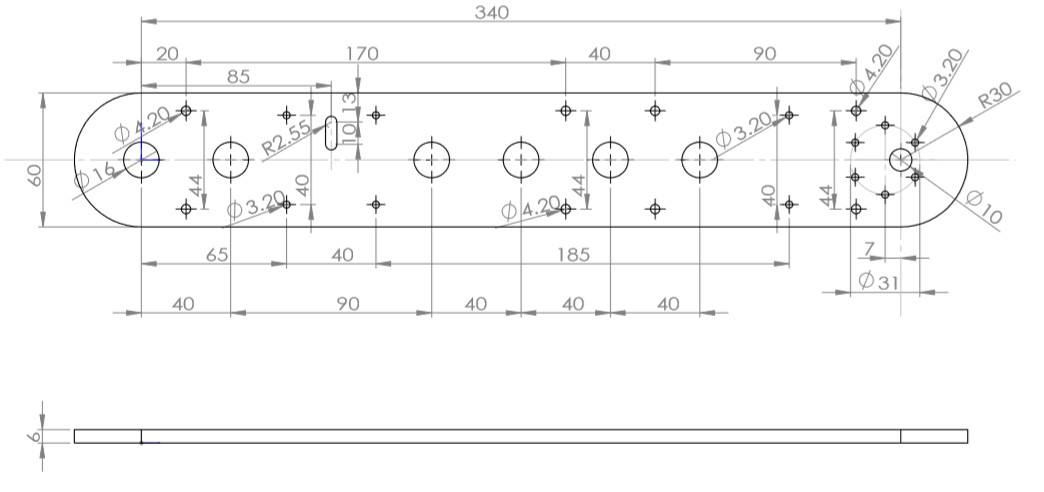
\includegraphics[width=.9\textwidth]{chap4//Fig3.jpg}
\caption{轴固定内板}
\end{figure}
 \begin{figure}[H]
\centering
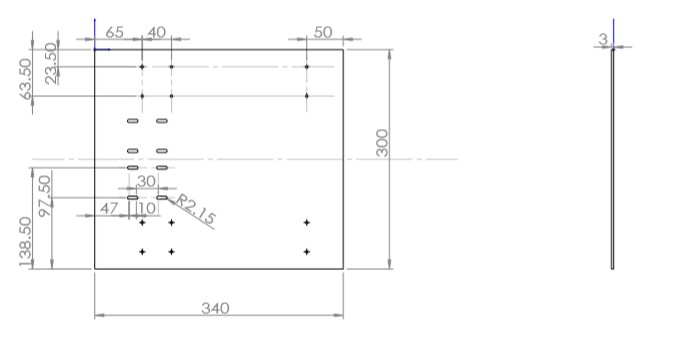
\includegraphics[width=.9\textwidth]{chap4//Fig4.jpg}
\caption{底板}
\end{figure}
\subsection{标准件选用}
\begin{itemize}
\item SN2H8固定环
\end{itemize}
由于成本原因,椭圆齿轮加工选择使用平板件激光切割,无法直接在零件上添加轴向与周向定位。使用SN2H固定环,侧边带顶丝孔,对椭圆齿轮进行一个定位。
\begin{figure}[H]
%\centering
\subfigure[SN2H8固定环  ]{
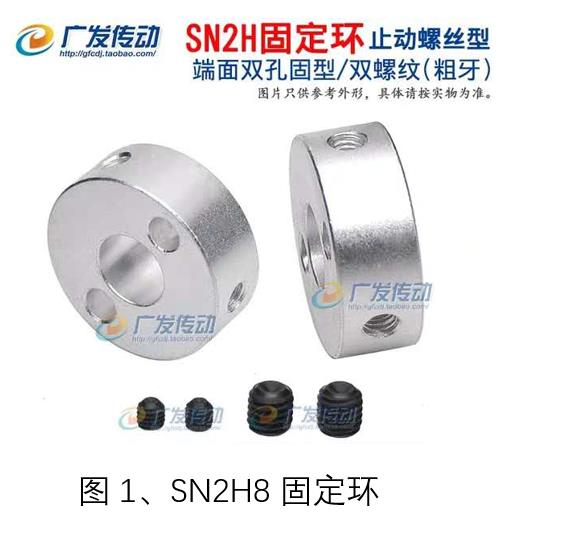
\includegraphics[width=.5\textwidth]{chap4//Fig5.jpg}
%\caption{fig1}
}
\quad
\subfigure[与椭圆齿装配]{
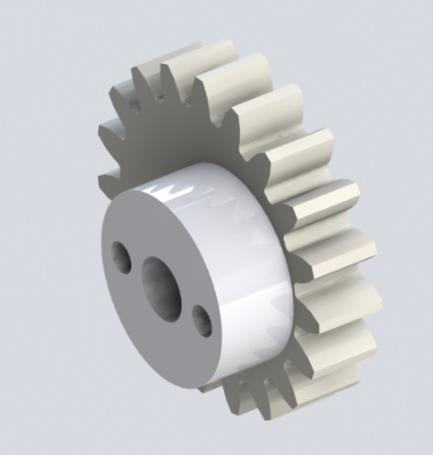
\includegraphics[width=.4\textwidth]{chap4//Fig6.jpg}
\quad
}
\caption{SN2H8固定环}
\end{figure}

\begin{itemize}
\item F688ZZ法兰轴承
\end{itemize}
由于轴固定板选用铝板激光切割,无法定位轴承。所以选用带法兰边轴承,用对轴进行一个定位,其优点在于自身带有一个单向的定位。
\begin{figure}[H]
%\centering
\subfigure[法兰轴承]{
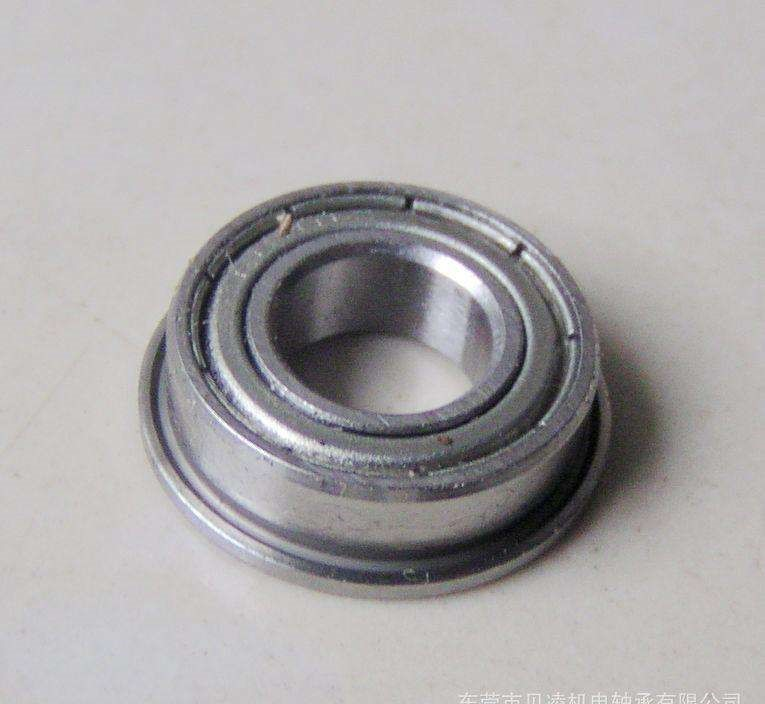
\includegraphics[width=.5\textwidth]{chap4//Fig7.jpg}
%\caption{fig1}
}
\quad
\subfigure[与轴板固定]{
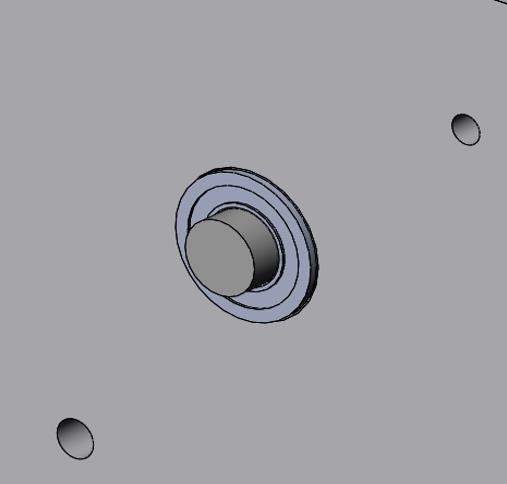
\includegraphics[width=.47\textwidth]{chap4//Fig8.jpg}
\quad
}
\caption{F688ZZ法兰轴承}
\end{figure}
\begin{itemize}
\item SCRH8固定环
\end{itemize}
由于未对轴进行开卡簧槽之类的加工,所以利用固定环起到一个固定轴以及轴承的作用
\begin{figure}[H]
%\centering
\subfigure[SCRH8固定环]{
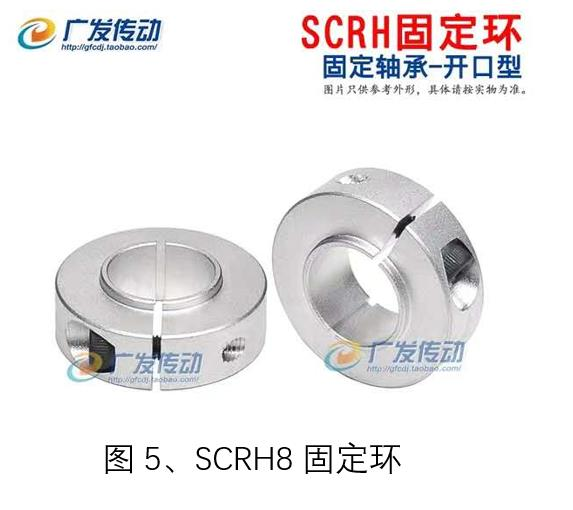
\includegraphics[width=.5\textwidth]{chap4//Fig9.jpg}
%\caption{fig1}
}
\quad
\subfigure[对轴进行固定]{
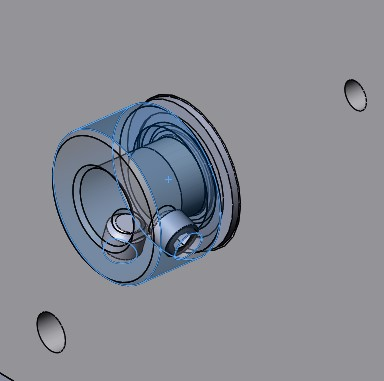
\includegraphics[width=.5\textwidth]{chap4//Fig10.jpg}
\quad
}
\caption{SCRH8固定环}
\end{figure}
\begin{itemize}
\item 凸台直齿轮
\end{itemize}
由于尺寸要求,齿轮系驱动前足大小齿轮分别选用1模25齿和30齿,经校核可以满足轮式运动状况下的载荷需求。同时,由于经费原因驱动前足所使用的轴均为光轴,为保证齿轮的轴向固定,选用可以利用紧定螺丝作为轴向固定的凸台齿轮。
\begin{figure}[H]
%\centering
\subfigure[齿轮尺寸示意图]{
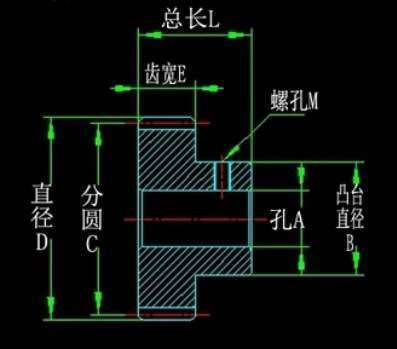
\includegraphics[width=.4\textwidth]{chap4//Fig11.jpg}
%\caption{fig1}
}
\quad
\subfigure[齿轮模型图]{
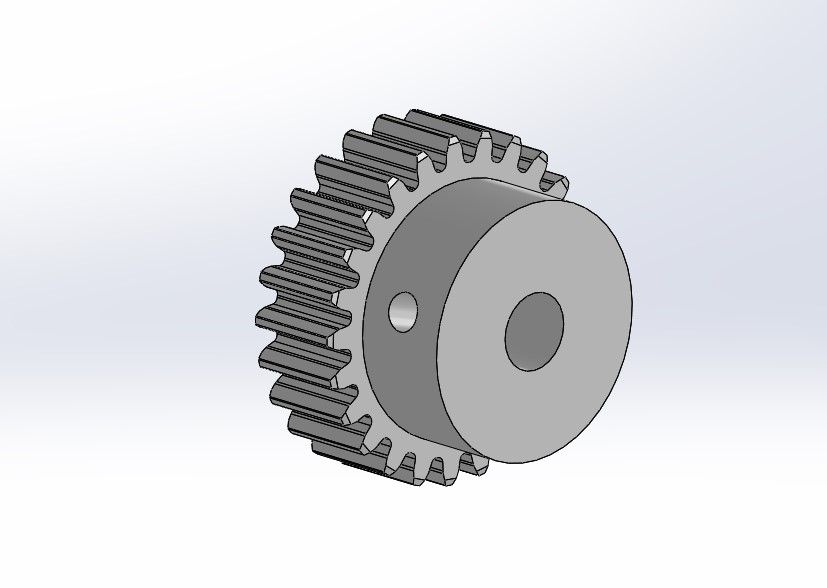
\includegraphics[width=.55\textwidth]{chap4//Fig12.jpg}
\quad
}
\caption{凸台直齿轮}
\end{figure}

\section{电控部分设计}
\subsection{总体概述}
\subsubsection{流程图}
 \begin{figure}[H]
\centering
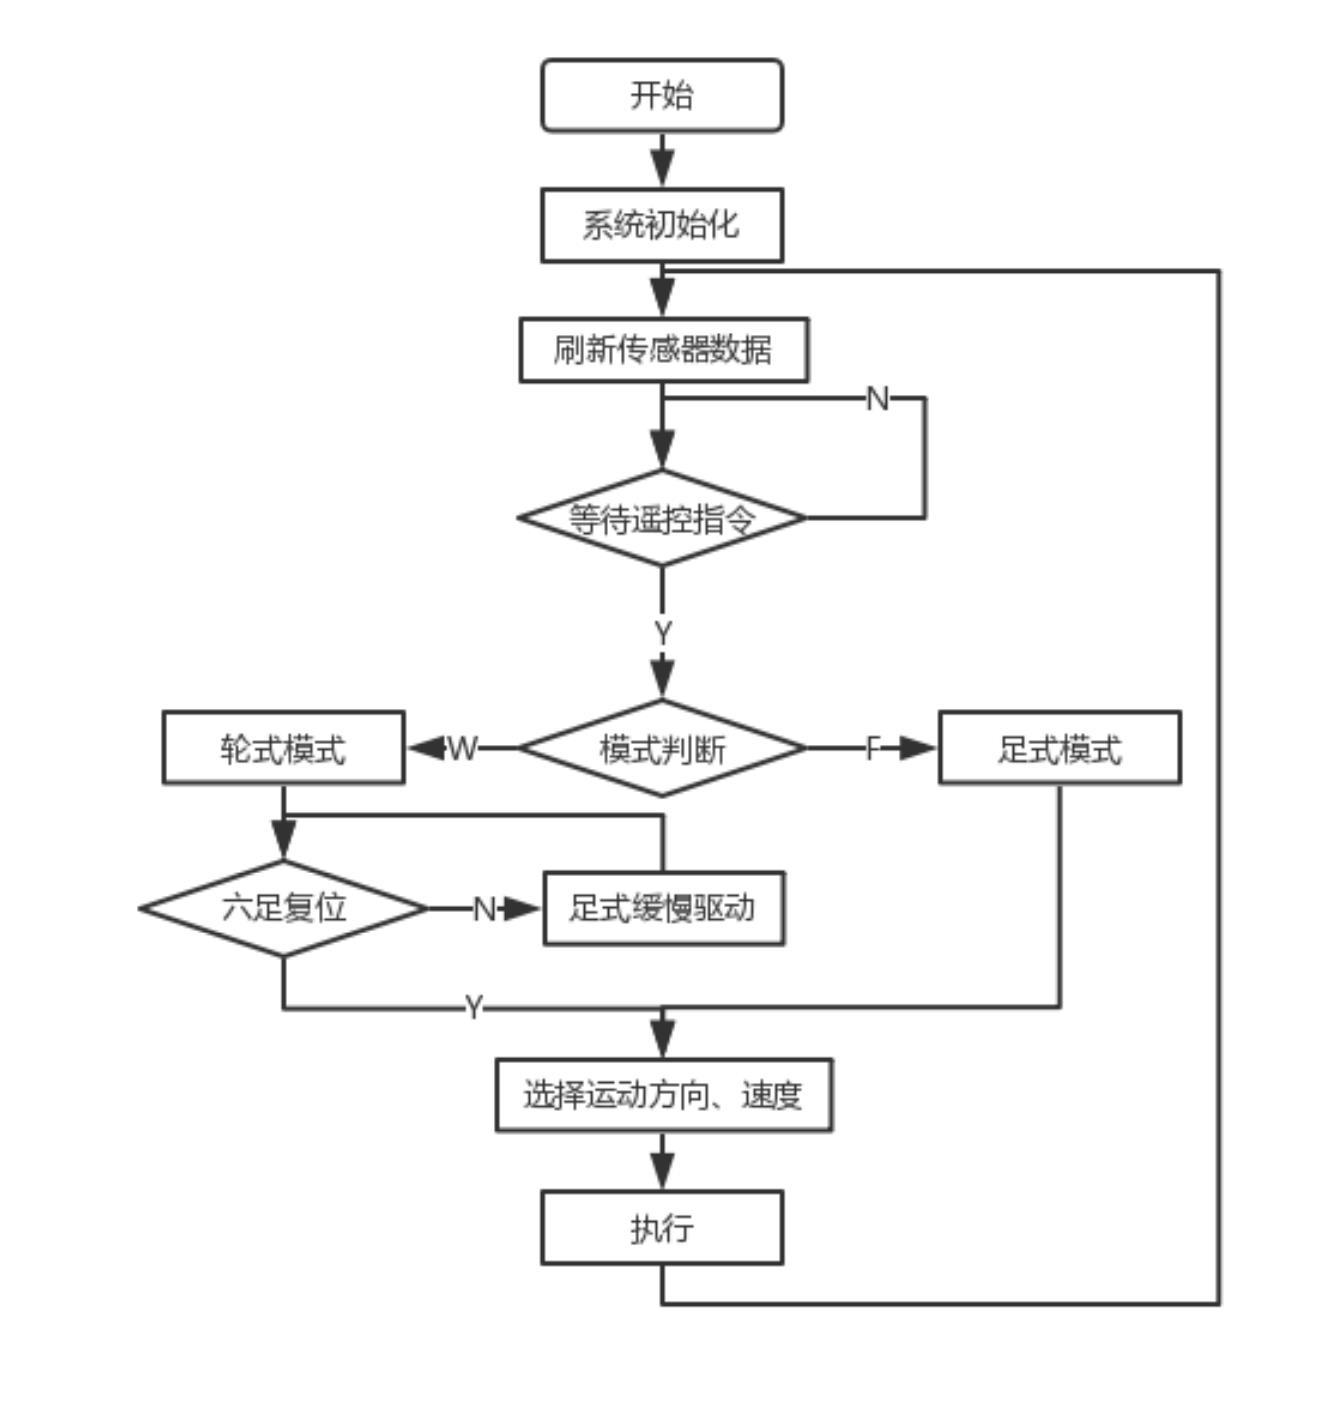
\includegraphics[width=.8\textwidth]{chap5//fig1.jpg}
\caption{控制流程图}
\end{figure}
\subsubsection{功能简介}
\begin{itemize}
\item 足式驱动
\end{itemize}\par
初始化:以两侧轮足平行的上电位置为基准,驱动其中之一侧,使之相差180°;\par
运行:同向同速驱动两侧轮足前进,反向同速驱动两侧旋转。
\begin{itemize}
\item 轮式驱动
\end{itemize}\par
初始化:驱动两侧轮足,使两侧前轮同时处于最低点;\par
运行:同向同速转动前轮前进,差速驱动转弯。

\begin{itemize}
\item 遥控部分
\end{itemize}\par
右上拨杆最上为轮式模式,此时左上拨杆控制高速、低速和停止,右侧摇杆上下推动控制前进后退,左右推动进行转弯;最下为足式模式,此时右侧摇杆上下推动控制前进后退,仅在无前后运动速度的情况下左右推动进行原地旋转控制;中间为停止状态,对任意输入不响应。
\subsubsection{电子器件}
 \begin{figure}[H]
\centering
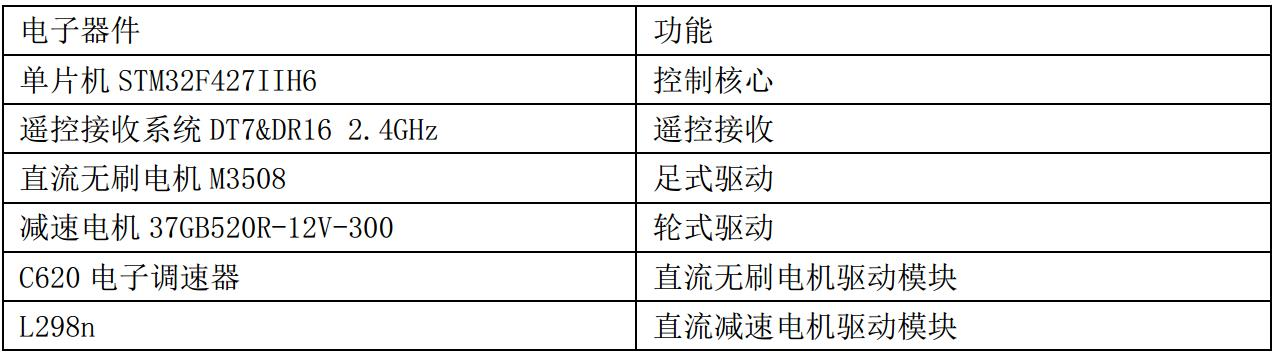
\includegraphics[width=.9\textwidth]{chap5//fig2.jpg}
\caption{电子器件清单}
\end{figure}
\subsubsection{操作系统配置}
 \begin{figure}[H]
\centering
\includegraphics[width=.77\textwidth]{chap5//fig3.jpg}
\caption{操作系统任务及其优先级}
\end{figure}

\subsection{硬件结构}
\subsubsection{硬件结构图}
 \begin{figure}[H]
\centering
\includegraphics[width=.95\textwidth]{chap5//fig4.jpg}
\caption{硬件结构框图}
\end{figure}
\subsubsection{主控板介绍}
该开发板主控芯片为STM32F427IIH6芯片,通过24v直流电源供电,板载可控电源输出,有丰富的扩展接口和通信接口,可以充分满足控制需求。在本项目中,用到了看门狗、定时中断,串口通信、CAN通信,GPIO、PWM接口。
 \begin{figure}[H]
\centering
\includegraphics[width=.8\textwidth]{chap5//fig5.jpg}
\caption{主控开发板}
\end{figure}
\subsubsection{动力输出介绍}
M3508无刷直流电机工作电压为24v,最高功率可达220w,最大扭矩5N*m,有感FOC控制在任何转速下都能提供稳定的扭矩,让机器人在快速响应的同时保持平稳的动力。带有编码器,配合C620电调使用,可以得到角度、速度、转矩、温度等参数,通过CAN总线控制,高效方便。该电机可自动感应高温、断线等异常并报警,同时反馈故障,使用安全。
37GB520R-12V-300直流减速电机工作电压为12v,额定力矩2.25kg*cm,通过PWM控制,可实现一定范围内的调速,但占空比直接影响输出电压,过低会使电机无法工作。
\subsection{控制系统}
\subsubsection{程序框架}
 \begin{figure}[H]
\centering
\includegraphics[width=.8\textwidth]{chap5//fig6.jpg}
\caption{程序框图}
\end{figure}
\subsubsection{指令层}
指令层为程序的顶层,该层又分为两部分:遥控器数据读取、整车运行状态机。以遥控器串口中断作为外部输入,是人机交互的接口部分,为了实现人对该六足机器人的控制,该中断为第一优先级,在任何时刻第一时间响应人的指令。\par
整车运行状态监测在定时器中断中进行,包括控制模式切换(足式运行模式、轮式运行模式、以及预留的自动模式)、运行状况状态机(开机启动初始化、电机堵转等应急反应、干扰或潜在bug的异常抛出),使整个控制条理清楚,为进一步开发预留了合理的空间。另外,该程序添加了IWG(看门狗复位),在意外情况下紧急重启,不会发生失控状况。
\subsubsection{控制层}
中间层为控制层,包括足式运行控制、轮式运行控制、红绿状态指示灯三个部分,控制层接收指令层的命令和处理驱动层反馈的数据。\par
对足式驱动电机采用经典的PID控制,主控板与电子调速器之间通过CAN总线通信,主控读取编码器值并解算得到角度、速度,以目标值与实际值之差为输入量,通过双闭环PID算法得到电流作为输出量即控制量,发出电流指令。对轮式驱动电机采用IO控制转向及锁死、PWM控制速度,设置高速、中速、低速三个档位。红绿状态指示灯按照状态机状态出现不同的闪烁情况。
\subsubsection{驱动层}
驱动层为程序底层,包括串口、定时器、CAN总线、GPIO等外设的初始化与驱动,实现与电子调速器之间的数据收发,串行通讯设备之间的数据收发,PWM波输出等底层驱动。在驱动层和控制层之间学习了骆学长的IOPool中间层进行数据交换,读写完全分离,保证了不会出现误修改问题。
\subsection{当前问题及改进方向}
\subsubsection{当前问题}
单侧轮足的耦合运动设计,使得该六足机器人在足式模式下不能实现差速转弯,否则将打乱两侧轮足相差180°的结构,使平台颠簸,损伤机器人。仅能采用原地旋转的方式进行原地转弯。\par
轮式驱动在前足,故如果同速反向驱动电机,机器人将会绕两前足中心旋转,而不是绕整个平台的中心旋转;由于后轮是单向旋转的普通从动轮,后轮在转动过程中会受到平行于轴的侧向力,引起较大的摩擦。\par
由于编码器是针对转子而言,且减速比为19:1,故如果运行过程中出现异常并重启,机器人将无法找到自己的当前位置,对两侧轮足的相对角度控制造成困难。
\subsubsection{改进方向}
针对以上第二个问题,可以根据尺寸和速度进行运动学解算,在旋转时给两轮进行速度补偿,使之绕平台中心旋转。\par
针对以上第三个问题,可以寻找合适的传感器,并找到合适的安装位置,来实现绝对位置的定位。比如磁电接触开关、触碰开关等。\par
说明,该工程为配套改装足式驱动电机为M3508后的程序,源码为文件“六足-stm32”,改自RoboMaster开源代码。 配套展示用42GA775F-12V-110直流电机的Arduino源码见文件“六足-Arduino”。\par
~\\
附,关键代码:
 \begin{figure}[H]
\centering
\includegraphics[width=.9\textwidth]{chap5//fig7.jpg}
\caption{双闭环PID角度、速度控制}
\end{figure}
 \begin{figure}[H]
\centering
\includegraphics[width=.9\textwidth]{chap5//fig8.jpg}
\caption{编码器溢出算法}
\end{figure}

\section{零部件报表}
\subsection{装配体视图}
 \begin{figure}[H]
\centering
\includegraphics[width=.81\textwidth]{chap6//fig1.png}
\caption{装配体多视角视图}
\end{figure}
 \begin{figure}[H]
\centering
\includegraphics[width=.85\textwidth]{chap6//fig2.png}
\caption{总装图}
\end{figure}
\subsection{BOM图}
 \begin{figure}[H]
\centering
\includegraphics[width=\textwidth]{chap6//fig3.png}
\caption{BOM图}
\end{figure}

\section{项目分工、感想}
\subsection{项目分工}
 \begin{figure}[H]
\centering
\includegraphics[width=1.2\textwidth]{chap7//fig1.jpg}
\caption{项目分工}
\end{figure}

\subsection{个人感想}
\textbf{严威:}\par
 
虽然说最终项目展的结果不尽如人意,但是对于我们小组最终能够完成实物的搭建和调试,我已经感到很满足了。\par
自己在一开始选题的时候意识到这样一个题目在后期的设计上可能会出现很多问题,但是实际上遇到的问题比预期的更加的多。比如说轴加工的问题,在初期设计的时候已经把传动轴的布置给设计完成了,当时以为只需要送加工就行了,结果拿到的报价却高的惊人,最终只能选择采用光轴的设计,又另外搜罗了很多方法进行一个定位。绘制椭圆齿轮时也是遇到了很大的麻烦,网上查阅的资料并不能很清楚的表述椭圆齿轮的整个绘制过程,造成一遍有一遍的尝试。齿轮系更是因为加工精度的问题出现过运转不流畅的问题。\par
由于这些可能说是意料之外又是情理之中的插曲,我们的每个零部件基本上都是经过了三到四版的改版才最终定稿。但就是这样仍然有很多的细节没有考虑到,影响到了最终的一个演示效果。\par
不过很幸运的是这次课程项目的组员们都很认真负责,身为一个组长不需要每天去催进度,只要在组会上确定了分工和各个项目的截止日期,大家无论个人能力如何,都会尽力在截止日期之前把手头上的任务做完。所以虽然整个设计过程中遇到了很多问题,但是现在回想起来没有什么感到特别崩溃的时候,发现问题-改良-再发现问题,整个设计过程还是比较流畅的。感觉这可能是团队合作最理想的状态了。\par
实话实话,得知项目展的结果自己确实是有点失望,但是很高兴的是自己的小作品得到了老师的认可。希望之后有机会的话,可以把结构改良一下,解决自己在初步设计过程中遇到的问题,获得更加好的一个运动效果。
\begin{figure}[H]
\centering
\includegraphics[width=0.3\textwidth]{photo//yw.jpg}
\caption{严威}
\end{figure}
~\\
\textbf{黄威:}\par

本此项目中,我前后参与了线驱动机械臂的设计、齿轮系驱动前足的设计与装配以及电控部分的调试。其中印象最深的有那么几个细节。\par
记得项目初期的几次答辩,盛老师要求每个项目先确定出基本的性能指标,并在此基础上对各个部分进行材料选型以及结构设计等等。相比起以往课程设计先制作最后再描述性能的过程,这样的要求是具有一定的挑战性的,但也的确是工程项目不可或缺的环节。从最后的结果来看,我们大概完成了预期目标的85$\%$,由于电机选型不当等原因最终没能实现全地形足式行进的预期目标,同时经费远远超出了预期。对于课程项目而言,这样的结果或许是可以接受的。但也应该注意到如果放在一个企业来看,百分之九十九就是零。无论是预期目标没有达到还是经费的超出都可能让先前所有的努力成为泡沫。这是在将来的项目中需要格外注意的。\par
其次,齿轮系驱动前足的制作也让我收获很多。因为尺寸限制以及零部件数量的原因,在设计过程中我们利用爆炸图等手段提前考虑了安装流程以及装配的可行性;将课程中学习到的知识运用到板材和齿轮的选型中。同时,也积极思考有创新性地提出齿轮系与平行四杆相结合的结构以及扭簧柔性约束等等。但项目中我们也遇到了由于标准件精度不够导致原本根据理论计算得到的齿轮中心距不能满足安装需求等问题,为将来做机械设计积累了经验。\par
最后,感谢盛鑫军老师以及张恒助教对我们项目提出的宝贵建议和指导,感谢队友的全勤投入和付出。
\begin{figure}[H]
\centering
\includegraphics[width=0.3\textwidth]{photo//hw.jpg}
\caption{黄威}
\end{figure}
~\\
\textbf{张芳园:}\par
本次项目给我带来很多收获,主要体现在标准化思想、灵活设计思维,机械与电控的配合,以及对合作更深入的理解三个方面。\par
在制作前足的过程中,我们尝试全部使用标准件,由于尺寸、重量和经费的极大限制,设计以及迭代过程都充满挑战,最终采用尼龙柱固定两板间距,分别依靠齿轮和固定环向两端顶紧的固定方式,将每一个零件按照要求进行装配,并进行必要的防松,使之不仅具有很高的还原度,而且有相对可靠的性能。扭簧约束、轴距微调、可调孔位、解耦设计、防锁死限位等等,每一处细节都是我们周密考虑的结果。\par
另外,在项目尾声阶段,我们发现减速电机扭力不够,以致于无法支撑六足机器人完整实现功能后,我们没有放弃,而是通过增加牛眼轮辅助实现足式运动,验证了机械结构的可行性,并决定改用性能更优的M3508电机将本项目做圆满。我在RoboMaster开源代码的基础上修改出了初版代码,在这个过程中,我发现了几个突出的问题,包括足式模式无法在行进中转弯以及轮式模式旋转中心不在几何中心等等,深刻意识到机械决定性能边界,更加激发了我对做好机械设计的热忱。\par
回首一个学期的合作我认识到,合作不是配合,正确的见解要坚持去落实,要积极争取想做的部分,不应当把热情消耗在机械重复中,有灵感更要有勇气去尝试。整个项目的合作过程非常平稳,组长对进度的把控也很稳健,在此感谢我的队友对队伍的积极贡献,感谢盛鑫军老师和张恒助教给予的帮助和鼓励。
\begin{figure}[H]
\centering
\includegraphics[width=0.3\textwidth]{photo//fyy.jpg}
\caption{张芳园}
\end{figure}
\textbf{庄一能:}\par
在本次的课程项目中我主要负责部分零件的绘制以及整体的组装工作,收获是肉眼可见的。\par
首先,本以为对建模软件SolidWorks还是有一定了解的,具体到实际要求时,经常出现的情况是遇到一个特殊的问题就需要特地到网上去查相关的用法,导致建模的过程不仅低效而且繁琐,可见对于一款软件来说,基本会用和熟练运用,两者之间存在着本质的差距。\par
由我负责的椭圆齿轮的设计,这一过程充满了教育意义,一开始还存在侥幸心理,设计不过是在网上对已有图纸的拷贝,事实上,真正用心去了解之后才发现非圆齿轮这一块需要很深的研究。最基础的,是对课内知识的贯通,为此,直齿轮这一章节的相关内容反复推敲的很多遍。比如渐开线齿廓,齿顶、齿根圆这些内容,在非圆齿轮上也是互通的,其次需要大量相关文献的查阅,为此也开阔了自己的眼界。两版的失败设计后最终在第三版能画出啮合适当的椭圆齿轮模型,还归功于组长严威的督促。\par
模型组装真正让我体会到了机械设计的重要,从模型到实体之间的路还很长。零件加工需要考虑到安装时的配合问题,课程项目经费有限导致的加工精度问题,这些都是很实际的、不动手完全想到不到的,可以说课程的最后两周时间,基本都花费在解决当时设计图纸时没注意到的小失误上。另外课程中也对加工零件的方法有了一定程度的认识。学机械不仅仅是要实现原本预定的功能,更重要的是,需要考虑到后续的过程,设计要设想到实现的合理性,出图要别人能看懂,加工要综合成本和安装效果,组装要考虑到运行时的效率。一个合格的项目设计需要对全局都有把控,而目前的境界还离得很远,走一步看一步的设计是需要杜绝的。\par
尽管最后课程项目取得的成绩不尽如人意,但作为一个学机械的学生来说,这一个交学费的过程还是很有必要的,且收获的经验是对得起自己的付出的。最后也由衷感谢其他的组员和自己的组长,张恒助教以及盛鑫军老师。
\begin{figure}[H]
\centering
\includegraphics[width=0.3\textwidth]{photo//zyn.jpg}
\caption{庄一能}
\end{figure}
\textbf{李响:}\par
这次活动参与给我留下了深刻的印象,组内的每一个成员都十分重视项目设计工作,并且能够按时完成任务,主动分担项目进度的压力。项目受限于经费的压力和经验的不足,整体装配进行了两个周的时间,各个模块反复拆装,终于在大家齐心协力相互配合的情况下完成了装配的任务。我们项目进度受到了组长的严格把关,保证了最后的正常行走正常。\par
在进行项目的实施过程中,我学会了使用3D画图软件solidworks,来绘制相关的零部件图形,并且积极与组长沟通零件的尺寸大小和材料选择,最终负责了有关于C型足的设计与采购部分,通过联系多个商家确定了购买的对象,在价格与质量上做出了权衡和比较。\par
项目中间阶段由于受到了其他的课程中期考试的影响,自己出现了懈怠的情绪,在组长的及时督促下和组内成员的相互鼓励下,完成了每一次课上答辩任务。
老师要我们每个周都要有计划的实施相应的工作,我们每个周都要保证相应的计划实施,因此,我们的课程项目虽说有些延迟,但是如期完成了任务。反思到自己积极参与了项目的整个制作过程,因此得到了很大的提升。

\begin{figure}[H]
\centering
\includegraphics[width=0.3\textwidth]{photo//lx.jpg}
\caption{李响}
\end{figure}
\newpage
\section{总结}
\subsection{项目创新点}
\subsubsection{C形足传动部分}
\begin{itemize}
\item 使用单个电机控制3个C形足的运动,实现单输入多输出的控制模式,降低了控制难度,节省了整机成本。
\item 使用椭圆齿轮产生急回效应,相较于连杆结构更加紧凑,提升运动性能。
\end{itemize}
\subsubsection{齿轮系前足部分}
\begin{itemize}
\item 结合齿轮系与平行四杆机构实现可变轴距传动,完成轮式前行。
\item 添加关节扭簧,限制自由度的同时,提供一定的缓冲效果,抵抗在崎岖地面上遇到的冲击载荷。
\end{itemize}
\subsection{项目改进}
\subsubsection{质量问题}
首先需要提及质量,质量可以说是此类结构的一大硬伤。目前,我们设计的整车重量为8kg,比预计的6kg还是多出2kg,直接导致了运动性能降低,也是电机无法驱动的一个主要问题。\par
同时,之所以产生C形足的设计,是因为如果C形足本身采用复合材料等具有较高弹性及韧性的材料,在车身较轻的前提下,是可以实现一种跳跃的效果的,对于其翻越沟渠具有较大的帮助。\par
由于我们项目设计采用了大量的齿轮及同步轮结构,造成基础重量比较重,如果想要减重,可以通过镂空和替换材料来实现。

\subsubsection{电机扭矩校核}
在项目初期没有进行电机的校核,可以说本次项目最大的失误了,通过后期的扭矩校核,发现一开始选择电机根本无法实现基础的足式运动。\par
所以打算更换直流有刷电机为直流无刷电机,增大减速度,以满足平地的足式运动以及翻越台阶等一系列乐章操作。

\subsubsection{运动问题}
项目设计的本身目的是想通过减少驱动电机来实现逻辑算法的简化,这个出发点本身没有错,但在后期的建模和演示过程中发现,靠普通的直流电机,单纯利用正反转其实没有办法让平台在足式运动时保持一个较为平稳的状态。\par
        所以如果后期进一步改进,我们想要使用无刷直流电机配备编码器,能够获得角度反馈。同时,在平地运动时的足式运动算法和爬越台阶时的运动算法也应该存在差异,实现一个运动的优化,减少在爬越台阶时候电机承受的一个转矩。

\subsubsection{定位问题}
由于成本问题,我们所有的轴都是采用 光轴,轴上零件多利用顶丝和抱紧进行轴向和周向地位,造成的直接影响是在大转矩的情况下,轴上零件可能出现打滑的现象,造成运动的失真。\par
如果后期进一步改进,需要设计阶梯轴,添加更为可靠的周向定位方式,来适应大转矩的运动场合。

\subsubsection{运动效率}
我们初期时设计轮式运动的目的是为了能够在平地上利用轮式运动来提高运动效率,增加平台的稳定性。\par
但实际上由于结构本身的限制,驱动轮的半径不可能做的非常的大,造成运动速度收到机械结构的一个限制,不能够非常快速的前进。

\subsubsection{整体机械结构的稳定性}
可以明显的发现,我们前轮的齿轮系是一个开式传动,而我们需要适应的地形恰好具有较高的复杂性和不确定性。并且,如果为了减重进行了镂空,那么污染物很容易通过空隙进入机体内部,影响其控制电路。\par
针对开式的齿轮传动,我想的是能不能利用一些壳体,对于不产生相对运动的部分进行一个包裹。对于会产生相对运动的关节扭簧处,则可以利用橡胶或波纹管类似的可伸缩材质进行一个包裹;针对镂空产生的污染物进入,我想能不能通过设计二层外壳进行污染物的隔离,这个二层外壳可以利用一些轻质材料进行制作,只需要起到隔离外界的作用。

\subsubsection{功能模块的配合}
 这个项目在设计过程中并没有考虑和设计一些外接设备的安放位置和接口,所以如果需要安放一些摄像头或者机械手的话可能需要额外设计空间进行一个搭载。
 \newpage
\section{致谢}
感谢盛鑫军老师在这一学期中各个阶段对我们项目的指导和点拨;\par
感谢张恒助教一学期以来对于我们的帮助和支持;\par
此外,也感谢学校工程训练中心提供的场地和工具支持。
\end{CJK}
\end{document}


 